% For tips on writing the thesis, see http://www.tug.org/pracjourn/2008-1/mori/mori.pdf

% Two side to save paper
% openrigth means to put the chapter tittle on the right pages
\documentclass[12pt,letterpaper,twoside,openright]{book}
\usepackage[utf8x]{inputenc}
\usepackage[T1]{fontenc}
% Language support
\usepackage[english,spanish]{babel}

\usepackage[table,xcdraw]{xcolor}


\newenvironment{dedication}
{
   \cleardoublepage
   \thispagestyle{empty}
   \vspace*{\stretch{1}}
   \hfill\begin{minipage}[t]{0.66\textwidth}
   \raggedright
}%
{
   \end{minipage}
   \vspace*{\stretch{3}}
   \clearpage
}

\newenvironment{acreditation}
{
   \cleardoublepage
   \thispagestyle{empty}
   %\vspace*{\stretch{1}}
   
   %\raggedright
}%
{
   
   %\vspace*{\stretch{3}}
   \clearpage
}


\newenvironment{notetoeditor}
{
   \begin{tcolorbox}[title={Nota al editor},colback=yellow!5!white]
}%
{
   \end{tcolorbox}
}

\newcommand*{\captionsource}[2]{%
	\caption[{#1}]{%
		#1%
		\\\hspace{\linewidth}%
		\textbf{Source:} #2%
	}%
}

\setcounter{tocdepth}{4}
\setcounter{secnumdepth}{4}

\selectlanguage{english}
%\usepackage[spanish]{datetime}

% We define some strings that will use along
\def \thesiskeywords {thesis, master degree, your topics here}
\def \pdfauthor {Student Name Here}
\def \thesistitle{Thesis Proposal Title Goes Here}

% Custom-commands and definitions
% See this file for defining the keywords that will show up on the PDF file
%For spanish we need indentation on the first line
%\usepackage{indentfirst}

%math package
\usepackage{amsthm}
\usepackage{amsmath}
\usepackage{amssymb}
\usepackage{pseudocode}

\newcommand{\lstnumberautorefname}{Listing}


\newtheorem{definition}{Definition}[subsection]
\newcommand{\definitionautorefname}{Definition}

\newtheorem{theorem}{Theorem}[subsection]
\newtheoremstyle{theorem}{}{}{\itshape}{}{\bfseries}{.}{.5em}{\thmnote{#3's }#1}
\newcommand{\theoremautorefname}{Theorem}

\newtheorem{lemma}{Lemma}[subsection]
\newtheoremstyle{lemma}{}{}{\itshape}{}{\bfseries}{.}{.5em}{\thmnote{#3's }#1}
\newcommand{\lemmaautorefname}{Lemma}

\newtheorem*{remark}{Remark}
\newcommand{\remarkautorefname}{Remark}

\newcommand{\algorithmautorefname}{Algorithm}

\usepackage{listings}

\lstdefinestyle{customc}{
  language=C++,
  belowcaptionskip=1\baselineskip,
  breaklines=true,
  frame=l,
  xleftmargin=\parindent,
  showstringspaces=false,
  basicstyle=\linespread{0.9}\scriptsize,
  emptylines=0,
  keywordstyle=\scriptsize\ttfamily\bfseries\color{blue!40!black},
  commentstyle=\mdseries\scriptsize\color{gray!40!black},
  identifierstyle=\scriptsize\ttfamily\color{darkgray!15!black},
  stringstyle=\scriptsize\ttfamily\color{green!40!black},
}

\lstset{style=customc}

\usepackage{textcomp}
\DeclareUnicodeCharacter{8208}{fi}

\usepackage{supertabular}

%tables
\usepackage{multirow}
\usepackage{booktabs}
%\usepackage[table]{xcolor}

%figures in the exact position as code
\usepackage{float}

% Prevent latex from expanding to fill page
\raggedbottom

%Use the margins requested
\usepackage[hmargin={3.5cm,2.5cm},vmargin=2.5cm]{geometry}

%bold font for caption
\usepackage[labelfont=bf]{caption}

%\usepackage{digsig}

%Improved bibliography
\usepackage[round,sort,numbers,authoryear]{natbib}
\usepackage{usebib}
\bibpunct{[}{]}{;}{n}{,}{,}

% To define spacing
\usepackage{setspace}

% Bible references
\usepackage{verse}
\usepackage{bibleref}

% We use these packages for making the nice logo on the title page
\usepackage[pdftex]{graphicx}

%chemical
\usepackage{chemformula}

% Use input characters instead of scape codes
\usepackage[utf8x]{inputenc}

% Generate fancy chapter titles
\usepackage[Sonny]{fncychap}
\ChNameAsIs
\ChNumVar{\Large}
\ChNameVar{\fontsize{50}{60}}

%no word breaking
%\usepackage[none]{hyphenat}
\tolerance=1
\emergencystretch=\maxdimen
\hyphenpenalty=10000
\hbadness=10000

%Use Fancy headers
\usepackage{fancyhdr}
%\pagestyle{fancy}
%\fancyhead[LO]{\nouppercase{\leftmark}}
\lhead{\nouppercase{\rightmark}}

% Generate pretty PDF with links on the TOC
\usepackage{mdwlist}
\usepackage{alltt}
\usepackage[bookmarks=true,linktoc=all, colorlinks=true, pdftitle={\thesistitle}, pdfauthor={\pdfauthor}, pdfsubject={\thesistitle}, pdfkeywords={\thesiskeywords},
linkcolor=darkgray,filecolor=darkgray,urlcolor=darkgray,citecolor=darkgray]{hyperref}


\addto\extrasenglish{%
  \renewcommand{\chapterautorefname}{Chapter}%
  \renewcommand{\sectionautorefname}{Section}%
  \renewcommand{\subsectionautorefname}{Section}%
  \renewcommand{\subsubsectionautorefname}{Section}%
}

\newcommand*{\fullref}[1]{\hyperref[{#1}]{\autoref*{#1}, \nameref*{#1}}} % One single link

\newcommand*{\listingref}[1]{\hyperref[{#1}]{\autoref*{#1} \nameref*{#1} [page~\pageref{#1}]}}

% Allow epigraphs at the beginning of chapters
\usepackage{epigraph}
\setlength{\epigraphrule}{0pt}
\setlength{\afterepigraphskip}{10pt}

% Define abstract environment since it doesn't exists on book class
\newenvironment{abstract}%
{\cleardoublepage\null \vfill \begin{center}%
\bfseries \abstractname \end{center}}
{\vfill\null}

% Generation of nomenclature
\usepackage{nomencl}
\makenomenclature

% Generation of acronyms
\usepackage[footnote,withpage,printonlyused]{acronym}

% For color definitions
\usepackage{color}

% Comment this out when is not a draft
%\usepackage{draftwatermark}
%\SetWatermarkLightness{0.95}
%\SetWatermarkFontSize{5cm}
%\SetWatermarkScale{5}
%\SetWatermarkText{DRAFT}

% Custom commands
\newcommand{\HRule}{\rule{\linewidth}{0.5mm}}

\usepackage{cclicenses}

\usepackage{soulutf8}
\usepackage{varwidth}

\definecolor{light-gray}{gray}{0.75}

\newcommand\backBox[1]{%
  \colorbox{light-gray}{\begin{varwidth}{\dimexpr\linewidth-2\fboxsep}#1\end{varwidth}}}
  
\newcommand\hightligher[1]{%
  \colorbox{yellow}{\begin{varwidth}{\dimexpr\linewidth-2\fboxsep}#1\end{varwidth}}}
  
  
\usepackage{tcolorbox}
\usepackage{tabularx}
\newcolumntype{L}{>{\raggedright\arraybackslash}X}
\usepackage{array}
\usepackage{colortbl}

\newcolumntype{Y}{>{\raggedleft\arraybackslash}X}

\tcbset{tab1/.style={fonttitle=\bfseries\large,fontupper=\normalsize\sffamily,
colback=white!10!white,colframe=red!75!black,colbacktitle=white!40!white,
coltitle=black,center title,freelance,frame code={
\foreach \n in {north east,north west,south east,south west}
{\path [fill=gray!75!black] (interior.\n) circle (3mm); };},}}

\tcbset{tab2/.style={fonttitle=\bfseries,fontupper=\normalsize\sffamily,
colback=white!10!white,colframe=gray!50!black,colbacktitle=white!40!white,
coltitle=black,center title}}

\usepackage{pgfgantt}
\usepackage{soul}
%\include{eshyph.tex}
\usepackage{tikz}
\usepackage{verbatim}
\usetikzlibrary{calc,trees,positioning,arrows,chains,shapes.geometric,%
    decorations.pathreplacing,decorations.pathmorphing,shapes,%
    matrix,shapes.symbols}

\tikzset{
>=stealth',
  punktchain/.style={
    rectangle, 
    rounded corners, 
    % fill=black!10,
    draw=black, very thick,
    text width=10em, 
    minimum height=3em, 
    text centered, 
    on chain},
  line/.style={draw, thick, <-},
  element/.style={
    tape,
    top color=white,
    bottom color=blue!50!black!60!,
    minimum width=8em,
    draw=blue!40!black!90, very thick,
    text width=10em, 
    minimum height=3.5em, 
    text centered, 
    on chain},
  every join/.style={->, thick,shorten >=1pt},
  decoration={brace},
  tuborg/.style={decorate},
  tubnode/.style={midway, right=2pt},
}

\usepackage{pdflscape}
\usepackage{svg}

% TODO List support

\usepackage{xargs}                      % Use more than one optional parameter in a new commands

\usepackage{algorithm}
\usepackage[noend]{algpseudocode}


\usepackage[colorinlistoftodos,prependcaption,textsize=tiny]{todonotes}
\newcommandx{\unsure}[2][1=]{\todo[linecolor=red,backgroundcolor=red!25,bordercolor=red,#1]{#2}}
\newcommandx{\change}[2][1=]{\todo[linecolor=blue,backgroundcolor=blue!25,bordercolor=blue,#1]{#2}}
\newcommandx{\addsummary}[2][1=]{\todo[linecolor=yellow,backgroundcolor=yellow!25,bordercolor=yellow,#1]{Add summary of: #2}}

\newcommandx{\addmoreinfo}[2][1=]{\todo[linecolor=yellow,backgroundcolor=yellow!25,bordercolor=yellow,#1]{Add more information about: #2}}

\newcommandx{\rewritethis}[2][1=]{\todo[linecolor=pink,backgroundcolor=pink!25,bordercolor=pink,#1]{Rewrite: #2}}

\newcommandx{\improvement}[2][1=]{\todo[linecolor=green,backgroundcolor=green!25,bordercolor=green,#1]{#2}}
\newcommandx{\thiswillnotshow}[2][1=]{\todo[disable,#1]{#2}}


\newcommand{\presentationitem}[1]{%
\iftoggle{paper}
{
  \subsubsection{#1}
}
{
  \item
  \def\@currentlabelname{#1}%
  \textbf{#1}
}
}

\newcommand{\presentationitembig}[1]{%
\iftoggle{paper}
{
  \subsection{#1}%
}%else
{%
  \item%
  \textbf{#1:}%
  \def\@currentlabelname{\emph{#1}}%
}
}


\newenvironment{wbstaks}
{
}
{
}

\newcommand{\presentationbreak}{}

\usetikzlibrary{decorations.text,calc,arrows.meta}


\usetikzlibrary{lindenmayersystems,arrows.meta}
\newcount\quadrant
\pgfdeclarelindenmayersystem{cayley}{
  \rule{A -> B [ R [A] [+A] [-A] ]}
  \symbol{R}{ \pgflsystemstep=0.5\pgflsystemstep } 
  \symbol{-}{
    \pgfmathsetcount\quadrant{Mod(\quadrant+1,4)}
    \tikzset{rotate=90}
  }
  \symbol{+}{
    \pgfmathsetcount\quadrant{Mod(\quadrant-1,4)}
    \tikzset{rotate=-90}
  }
  \symbol{B}{
    \draw [dot-cayley] (0,0) -- (\pgflsystemstep,0) 
       node [font=\footnotesize, midway, 
         anchor={270-mod(\the\quadrant,2)*90}, inner sep=.5ex] 
           {\ifcase\quadrant$a$\or$b$\or$c$\or$d$\fi};
    \tikzset{xshift=\pgflsystemstep}
  }
}
\tikzset{
  dot/.tip={Circle[sep=-1.5pt,length=3pt]}, cayley/.tip={Stealth[]dot[]}
}



\newtoggle{paper}
\settoggle{paper}{true}

\usepackage{csvsimple}


\begin{document}

% This is the first part of the document (frontmatter), use Roman numeration
\frontmatter

% Simple style
\pagestyle{empty}

% The front page of the thesis is in this page, Name of the school and the program can be changed here. Supervisor name gets changed here.
\selectlanguage{english}
\begin{titlepage}

\begin{center}

\vfill



\includegraphics[width=1\textwidth]{../images/TECRGB.jpg}
\\[0.2cm]
\definecolor{tecblue}{rgb}{0.016,0.173,0.322}
\textcolor{tecblue}{
\textsc{\LARGE Escuela de Ingeniería en Computación}\\[0.2cm]
\textsc{\large Programa de Maestría en Computación}\\
}
\vfill
 
% Title
\HRule
\\[0.9cm]
\doublespacing
{ \huge \bfseries \thesistitle}
\\[0.4cm]
\singlespacing
\HRule
\\[0.9cm]

{\large Thesis proposal submitted in partial fulfilment to opt for the degree of 
\\[1cm]
\textit{Magister Scientiæ} in Computer Science}
\\
\vfill
 
 % Author and supervisor
\begin{minipage}{0.45\textwidth}
\begin{flushleft} \large
Author\\
\pdfauthor 
\end{flushleft}
\end{minipage}
\begin{minipage}{0.50\textwidth}
\begin{flushright} \large
Supervisor\\
{Supervisor Name Here, Sup. Title}
\end{flushright}
\end{minipage}
 
 
\vfill
 
% Bottom of the page
{\large \today \\}  \hfill{} 

%\cludegraphics{../imagenes/cc.png} \\
%Liberado con una licencia Creative Commons Atribución, Compartir igual.

\end{center}
\end{titlepage}

%\digsigfield{5cm}{3cm}{julatec}

%

\selectlanguage{spanish}
%\begin{acreditation}
% The ghesis act goes here.
%\makebox[\linewidth]{
    
\includegraphics[width=0.75\paperwidth,height=1\paperheight]{../images/certificate.pdf}
%}

%\end{acreditation}

% The abstract is included on a separte file here
\newpage
\thispagestyle{empty}
\mbox{}

% Now let put the abstract in two languages
\doublespacing

\selectlanguage{english}%
\begin{abstract}
\iftoggle{paper}
{
The body of the abstract goes here.
 
}%


\end{abstract}

%\selectlanguage{spanish}%
%\begin{abstract}
%\input{body/resumen-text}
%\end{abstract}

\selectlanguage{english}


%\singlespace


%Table of contents is generated here
\tableofcontents

%List of figures goes here
\listoffigures

%List of tables is generated here
\listoftables

\mainmatter
% Use double space
\doublespacing
% Now fancy style
\pagestyle{fancy}
\setlength{\headheight}{14.5pt}
% Left the right header clean
\rhead{}

\renewcommand{\chaptername}{Chapter}

\doublespacing

% The section introduction is included
\chapter{Introduction}
\label{chapter:introduction}


Introduction section goes here. Here is an example reference
\cite{examplereference}. Here is another example reference \cite{examplereference2}.

\newpage

\section{Problem}

Problem context, description and summary goes in this section

\section{Document Structure}

Provide a brief explanation of the intent of this document, as well as what has been described in the current section. Then describe what is included in each one of the sections. 




% Theoretical framework contents
\chapter{Theoretical Framework}
\label{chapter:theoretical-framework}


This chapter describes the theoretical concepts needed to understand the work that will be developed during the research's execution.


\section{Concept 1}

\label{section:Concept1}

First theoretical framework concept goes here.

\subsection{Subsection of Concept 1} 
\subsection{Subsection 2 of Concept 1}
Some text goes here \cite{examplereference}. An example of displaying and referencing an image is shown in \textbf{Figure \ref{fig:example}}


\begin{figure}
	\begin{center}
		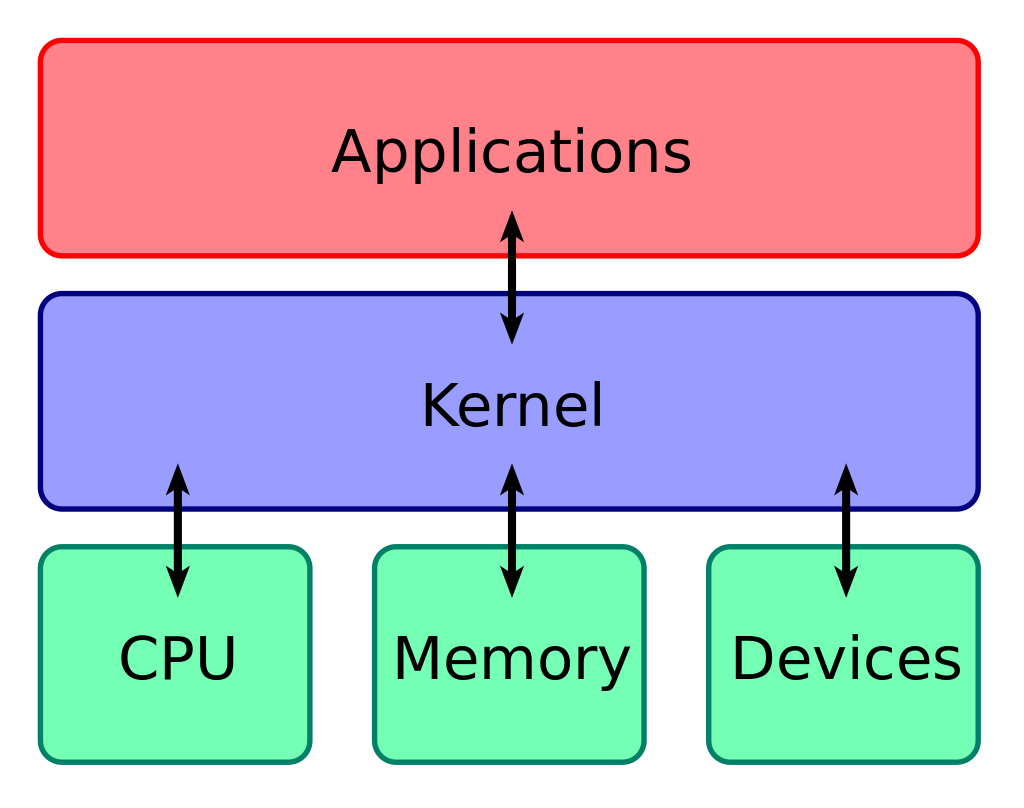
\includegraphics[width=1\columnwidth]{../img/image.png}
		\caption[]{Example image with reference \cite{examplereference}.}
		\label{fig:example}
	\end{center}
\end{figure}


\section{Concept 2}

\label{section:Concept2}

\subsection{Subsection Concept 2}

\subsubsection{Subsection 2 Concept 2}

\section{Concept 3}
An example of pseudo-code can be seen in \textbf{Algorithm \ref{examplepseudocode}}

\begin{pseudocode}{Pseudo\_Code}{Input} \label{examplepseudocode}
	\FOR y \GETS 1 \TO Input.MaxL \DO
	\BEGIN
	\FOR x \GETS 1 \TO Input.MaxH \DO
	\BEGIN
	a \GETS \CALL {FunctionCall}{x,y}\\
	b \GETS \CALL {AnotherFunction}{x, y}\\
	\CALL {ThirdFunction}{a,b}
	\END
	\END
\end{pseudocode}


\subsection{Example equation}
 Equation \ref{eq:1} shows an example equation.

\[
I=(L\cdot N) \tag{1} \label{eq:1}
\]
  
\section{Related Work}
The related work for the research is include in this section \cite{examplereference}.

% Hypothesis and objetives.
\chapter{Hypothesis and Objectives}
\label{chapter:hypothesis-objectives}
Example text:

This chapter presents the hypothesis formulated for the thesis. Also, it displays the established objectives with its corresponding deliverables. Last section gives a summary of the scope and limitations defined for this research.

\section{Hypothesis}
\label{section:hypothesis}
A brief context description of the formulation of the hypothesis can go here, followed by.
The hypothesis for this research effort reads as follows (example):

``Our proposed method $P$ in the research can improve by $Q$\footnote{If numbers are involved, usually an explanation of why that specific number was used is given in a footnote \cite{examplereference2}.} the relation in metric 1 and metric 2\footnote{The \cite{examplereference} definition of is used.}.''

\section{Objectives}
\label{section:objectives}
The current research established the following objectives:

\subsection{Main Objective}
\label{section:main-objective}
\label{objective:main}
Main Objective Text.

\subsection{Specific Objectives}
\label{section:specific-objectives}

\begin{enumerate}
	\item Specific objective 1.
	
	\item Specific objective 2.
	
	\item Specific objective 3.
	
\end{enumerate}

\subsection{Deliverables}
Example text:
This section provides the deliverables assigned for each specific objective defined for the thesis.

\textbf{Specific Objective 1:}
Deliverable for specific objective 1. 

\textbf{Specific Objective 2:}
Deliverable for specific objective 2.

\textbf{Specific Objective 3:}
Deliverable for specific objective 3.

\section{Scope and Limitations}

Should include the scope and limitations of the developed research.

\textbf{Scope and limitation 1:} 

\textbf{Scope and limitation 2:}
 
\textbf{Scope and limitation 3:} 
% Research proposal
\chapter{Research Proposal}
\label{chapter:research-proposal}

\section{Design/Method/Algorithm/Mechanism Proposal}

Explain the proposed design/method/algorithm/mechanism. A diagram is usually beneficial for understanding how the proposal would work.
 
\section{Experiment Design}
\label{section:experiment-design}
Establish the experiment design that will be used to evaluate the hypothesis.
\section{Factors and Levels (if needed):}
Determine and describe the factors and levels that will be used in the experiment.

\section{Measures and Combinations of the Experiment (if needed)}

The example \textbf{Table \ref{tab:table}} summarizes the factors and levels used in the experiments.
\begin{table}[h]
	\caption{Example table.}
	\label{tab:table}
	\begin{center}
		\begin{tabular}{|l|l|l|l|l|}
			\cline{2-5}
			\multicolumn{1}{c|}{}	& \multicolumn{4}{c|}{Factor} \\ 
			\cline{2-5}
			\multicolumn{1}{c|}{}	& Factor 1 & Factor 2 & Factor 3 & Factor 4 \\ \hline
			Levels
			& Level 1 & Level 1	& Level 1  & Level 1   \\
			& Level 2 & Level 2  & Level 2 & Level 2 \\
			& Level 3 & Level 3 & Level 3 & Level 3 \\
			& Level 4 &    & Level 4  &   \\ 
			&  &    & Level 5  &   \\ 
			&  &    & Level 6  &     \\\hline
		\end{tabular}
	\end{center}
\end{table}

Justify the number of runs and repetitions defined for the experiment.


\section{Response Variable}
Description of the response variable used in the research.

\section{Experiment set-up}

\section{Data Recollection}

Description of the data recollection process. 

\section{Statistical Tool Used Description}

Include a section briefly explaining the statistical tool used to analyze the data from the experiments.
%Preliminary-results
\chapter{Preliminary Results}
\label{chapter:preliminary-results}

If available or relevant, present preliminary results in this section.

%schedule
\chapter{Conclusions and Future Work}

\label{chapter:schedule}

Include a table describing all activities that need to be performed during the research, as shown in \textbf{Table \ref{tab:tasks}}. Include a Gantt diagram like the one shown in \textbf{Figure \ref{fig:gantt}}.

\begin{table}
	\centering
	\renewcommand{\arraystretch}{1}
	\caption{Tasks to be executed}
	\label{tab:tasks}
	\begin{tabular}{|p{1.75cm} |p{13cm}|}
		\hline
		\bfseries  Task \# &\bfseries Description \\
		\hline
		\multirow{1}{*}{1} &
		Description of the task.  \\
		\hline
		\multirow{1}{*}{2} &
		Description of the task. \\
		\hline
		\multirow{1}{*}{3} &
		Description of the task. \\
		\hline
		\multirow{1}{*}{4} & Description of the task. \\
		\hline
		\multirow{1}{*}{5} & Description of the task.\\
		\hline
		\multirow{1}{*}{6} & Description of the task. \\
		\hline
		\multirow{1}{*}{7} & Description of the task. \\
		\hline 
		\multirow{1}{*}{8} & Description of the task. \\
		\hline
		\multirow{1}{*}{9} & Description of the task. \\
		\hline
		\multirow{1}{*}{10} & Description of the task. \\
		\hline
		\multirow{1}{*}{11} & Description of the task. \\
		\hline
		\multirow{1}{*}{12} & Description of the task.\\
		\hline
		\multirow{1}{*}{13} & Description of the task. \\
		\hline
		\multirow{1}{*}{14} & Description of the task. \\
		\hline
	\end{tabular}
\end{table}



\begin{figure}
	\begin{center}
		\begin{tabular}{@{}r}
			
			\begin{ganttchart}[ x unit=0.8cm, y unit chart = 0.5cm]{1}{17}
				\gantttitle{Weeks of a semesteer}{17} \\
				\gantttitle{01}{1}
				\gantttitle{02}{1}
				\gantttitle{03}{1}
				\gantttitle{04}{1}
				\gantttitle{05}{1}
				\gantttitle{06}{1}
				\gantttitle{07}{1}
				\gantttitle{08}{1} 
				\gantttitle{09}{1}
				\gantttitle{10}{1}
				\gantttitle{11}{1}
				\gantttitle{12}{1}
				\gantttitle{13}{1}
				\gantttitle{14}{1}
				\gantttitle{15}{1}
				\gantttitle{16}{1}
				\gantttitle{17}{1}
				
				\\
				
				\ganttbar{Task 1}{1}{2} \\
				\ganttbar{Task 2}{1}{2} \\
				\ganttbar{Task 3}{1}{2} \\
				\ganttbar{Task 4}{2}{3} \\
				\ganttbar{Task 5}{2}{3} \\
				\ganttbar{Task 6}{3}{5} \\
				\ganttbar{Task 7}{5}{6} \\
				\ganttbar{Task 8}{6}{9} \\    
				\ganttbar{Task 9}{6}{9} \\
				\ganttbar{Task 10}{6}{9} \\
				\ganttbar{Task 11}{9}{10} \\
				\ganttbar{Task 12}{10}{13} \\
				\ganttbar{Task 13}{1}{16} \\
				\ganttbar{Task 14}{17}{17} \\
			\end{ganttchart}
		\end{tabular}
		\captionsource{Gantt diagram example} {Author}
		\label{fig:gantt}
	\end{center}
\end{figure}
%Appendix

\chapter{Appendixes}
\label{chapter:appendixes}
If needed or relevant, appendixes go here.




% Final pages
\backmatter

% Use single space
\singlespacing

% Bibliography
\cleardoublepage
\renewcommand{\bibname}{References}

\refstepcounter{chapter}
\addcontentsline{toc}{chapter}{\bibname}
\bibliographystyle{plainnat}
\bibliography{mendeley}{}

\doublespacing



\end{document}
